\documentclass[../main.tex]{subfiles}

\begin{document}

\renewcommand{\labelitemi}{\ding{226}}
\renewcommand{\labelitemii}{\ding{227}}


\part{Introduction}
\label{part:intro:general}

\chapter{Neutrino physics}
Exploration of the neutrinos is relatively young but perspective direction of the research in the particle physics. Over the last 60 years since its first experimental observation lots of breakthroughs were made. Many of them have been awarded with notable prizes. All this speaks of the great interest of the community in this topic. Many puzzles are still unsolved, plenty of challenging experiments are ongoing.

In this chapter the history of the neutrino research will be overviewed (\autoref{sec:hist}) as well as the current studies and experiments (\autoref{sec:exp}). The topic of the neutrino oscillations (\autoref{sec:osc}) will be described in more details as the main subject of the current thesis.

\section{Historical overview}
\label{sec:hist}
The prerequisites of the neutrino existence were found in the beginning if the XX century. The spectrum of the electrons from the neutron decay (called $\beta$-decay) was measured as continuous but not discrete~\cite{Chadwick1914}. At that time the neutron decay was imagined as $n\to p+e$. Non-discrete spectrum provoked plenty of theories such as energy non-conservation (by N. Bohr) or existence of the new hypothetical particle (by W. Pauli~\cite{Pauli1930}). Later Enrico Fermi developed a complete theory of beta decay~\cite{Fermi1934}. In the modern notation the decay process was presented as $n\to p^++e^-+\bar{\nu}_e$. Where neutrino is noted as $\nu$.

\subsection{Discovery of the neutrino}
The experimental discovery of the neutrino was pretty challenging. Neutrinos are not taking part in the electromagnetic or strong interactions. The only way to detect them is a weak interaction. Based on the Fermi's theory the inverse beta decay process should exist that will allow the direct observation of the neutrino. But the expected cross-section for such process was estimated at the level of $10^{-44} cm^2$. That was about couple of dozen orders less then cross-sections of the processed that were usually observed in the experiments at that time. That's why the neutrino discovery happened only 26 years after the proposal of the new particle.

After the proposal of the new particle few indirect measurements were performed, but the direct observation still remained a challenge. The first successful neutrino detection were done by group leading by Frederick Reines and Clyde Cowan~\cite{Cowan1956}. They performed series of experiments trying to detect neutrino from the most powerful source at that time - nuclear power plant. Relatively brand new material a liquid scintillator was used as a target and detector. The inverse beta decay was used as a detection reaction:
\begin{equation}
\bar{\nu}+p\to n+e^+
\end{equation}
The positron shortly annihilates with emitting of photons. In order to suppress background the Cadmium isotope was added to the detector. Thus the neutrons would be also detected with reaction
\begin{equation}
n+{}^{108}Cd\to{}^{109m}Cd\to{}^{109}Cd+\gamma
\end{equation}
As the ${109m}Cd$ lifetime is few tens microseconds the signal will have the unique signature: positron annihilation, and after a known time delay the gamma ray emission. Both signals will come with the fix energies. Thus rare signal events could be easily separated from the variety of the backgrounds.

Such strategy lead to the successful discovery of the particle that supposed to be ``undetectable'' before.

\subsection{Neutrino and anti-neutrino}
\label{sec:anti}
Soon after the neutrino discovery the question of its equivalence with the anti-neutrino was risen. Neutrino was the only known fermion without electric charge. So it was the only candidate for such equivalence. Raymond Davis performed the attempt to detect neutrino interactions with induction either electron or positron~\cite{Davis1955}. He use a clear beam of anti-neutrinos fro the reactor. If both reactions~\autoref{eq:nu} and~\autoref{eq:antinu} were detected that would mean that the neutrino ant anti-neutrino are equal.

\begin{eqnarray}
\label{eq:nu}
\bar{\nu}+p\rightarrow n+e^+ \\
\nu+n\rightarrow p+e^-
\label{eq:antinu}
\end{eqnarray}

He used the nuclear reaction with chlorine proposed by the Pontecorvo $\nu+{}^{37}Cl\to e^-+{}^{37}Ar$ with further decay of the ${}^{37}Ar$ with $\tau_{1/2}=35 days$. Such reaction was not observed that meant that neutrino interacted in different way comparing to anti-neutrino.

Goldhaber performed other extremely interesting experiment trying to measure the neutrino helicity~\cite{Goldhaber1958}. The electron capture by the Europium atom was used. The produced excited atom of Samarium further decay with photon emission. The photon polarity strictly depends on the neutrino helicity, that's how the last could be measured.

\begin{align}
Eu+e^-\to\nu+&Sm^* \\ \nonumber
&Sm^*\to Sm+\gamma
\end{align}

Goldhaber found that neutrino has only left helicity.

\begin{bclogo}[couleur=blue!2, arrondi=0.1, logo=\bcinfo, nobreak=true]{Helicity, polarity, chirality}
Helicity is a projection of the spin onto the direction of the momentum.
\begin{equation}
h=\frac{\vec{s}\cdot\vec{p}}{\left|\vec{s}\right|\left|\vec{p}\right|}
\end{equation}

The helicity could be ``left'' or ``right'' that corresponds to the spin direction opposite or co-directed with momentum. For the massless particles helicity is Lorentz invariant. The polarization of the particle beam is a percentage of the particles with a given helicity. For example 50\% polarization means that half of the particles are ``left'' and half are ``right''.

The chirality is a more fundamental characteristic versus helicity. It is determined by whether the particle wave function transforms with a right- or left-handed representation of the Poincare group.

Massless fermions keep chiral symmetry, i.e. independent rotation of the left- and right- handed components doesn't affect the theory. For them the helicity is always the same as chirality.

The massive particles break the chiral symmetry explicitly. Also for the massive fermions helicity is never more equivalent to the chirality as one could choose the reference frame moving faster then the particle and inverse the helicity.
\end{bclogo}

Combining results from Davis and Goldhaber we could conclude that neutrino and anti-neutrino interact in the different way, their helicity is different. Thus we still have possibility to describe the neutrino and anti-neutrino as the same particle but with different helicity. Such formalism was developed long before the described experiments by Ettore Majorana~\cite{Majorana1937}. He found a particular solution of the Dirac equation.

\begin{equation}
\left(i\gamma^\mu\partial_\mu-m\right)\psi=0
\end{equation}

In particular case of fermions the particle could be described in terms of spinors

\begin{align}
i\gamma^\mu\partial_\mu\psi_L&=m\psi_R\\ \nonumber
i\gamma^\mu\partial_\mu\psi_R&=m\psi_L
\end{align}

In case of massless fermion, like neutrino in the Standard Model (\autoref{sec:sm}) such notation is called Weyl spinors with two components. If the fermion is massive it could be described with four component spinors but only if $\psi_L$ and $\psi_R$ are dependent. That's how the Majorana equation was obtained

\begin{equation}
i\gamma^\mu\partial_\mu\psi_L=m\mathcal{C}\bar{\psi_L}^{T}
\end{equation}

This equation works only in case $\psi=\psi^C$. It means that such approach is not suitable for any charge fermion as their charge conjugation states are different because of e.g. different electric charge. But the neutrino is a unique particle to which this approach may be applicable.

Is neutrino a Majorana fermion or a Dirac fermion is still an open question. Neutrino oscillation experiments are not sensitive to this difference. The only way at the moment to find if the neutrino is a Majorana fermion is to detect the neutrinoless double beta decay. Plenty of experiments are challenging in this study~\cite{Bilenky2015}.

\begin{bclogo}[couleur=blue!2, arrondi=0.1, logo=\bcinfo, nobreak=true]{Symmetries: C, P, T}
In particle physics there are three important symmetries: charge (C), parity (P) ant time (T).

Parity inversion (P) flip the sign of the spatial coordinate $\mathcal{P}\overrightarrow{r}=-\overrightarrow{r}$ . In the QFT it's described as $\mathcal{P}\lvert\psi\rangle=c\lvert\psi\rangle$. Where $c$ is the eigenvalue of $\mathcal{P}$. The parity violation means a process that change the eigenvalue of the parity transformation for some system. The theory of such process was developed by Lee and Yang~\cite{Lee1956} and found in the Wu's experiment~\cite{Wu1957}. The asymmetry of the outgoing electrons from the Cobalt with respect to the nucleus polarization was the nice and clear proof for the effect.

Charge symmetry (C) transform particle to its anti-particle. $\mathcal{C}\lvert\psi\rangle=\eta_{C}\lvert\bar{\psi}\rangle$, where $\eta_{C}$ is the eigenvalue of the transformation. The example of the eigenvalue non-conservation experimental observation could be found in~\cite{Gormley1968}.

Time transformation (T) inverse the time direction. After the discovery of the separate P and C violations the combined symmetry breaking became the puzzle.

As it will be a hint towards T-symmetry breaking. The CP-violation was observed in the neutral kaons oscillations process~\cite{Christenson1964}. Later such process was confirmed with the direct measurements of kaon decays~\cite{AlaviHarati1999}~and~\cite{Fanti1999}, B-meson decays~\cite{Aubert2001}~and~\cite{Abe2001}, D-mesons~\cite{Aaij2019}.

Together they form a CPT symmetry. It's proved that any Lorentz invariant local quantum field theory with a hermitian Hamiltonian must be invariant under CPT.
\end{bclogo}


\subsection{Different types of neutrino}
\label{sec:dublet}
The first neutrino detection was made using the reactor as a particle source. Such source is extremely powerful, but isotropic. For the precise measurements is will be extremely useful to gain the statistics with the focused particle beam. For this the accelerators could be used. The general idea is to use proton beam hitting the target for the massive meson production. The charged meson could be focused and further decay producing the focused neutrino beam with high intensity. The description of such scheme in the modern experiment could be found in~\autoref{ch:T2K:nu_beam}. First time such approach was used to determine if the neutrino has flavors~\cite{Danby1962}. The main idea of the experiment is to use the neutrino flux produced from the pion decay. Because of the mass difference between electron and muon and the fixed neutrino helicity (\autoref{sec:anti}) charged pion decays mainly to muon, e.g. $\pi^+\to\mu^++\nu$. The question is could neutrino be ``muon'' or ``electron''. The experiment showed clearly that the reaction~\autoref{eq:notallowed} is severely suppressed comparing the reaction~\autoref{eq:allowed}.

\begin{align}
\label{eq:allowed}
\nu_\mu+p&\rightarrow n+\mu \\
\nu_\mu+p&\nrightarrow n+e
\label{eq:notallowed}
\end{align}

That means that neutrino has flavors. It could be either produced or detected with the lepton of the same flavor. The existence of the different types of the neutrino confirmed the doublet structure of the leptons. This fact will play an important rope in the theory of the neutrino oscillations.


\subsection{Neutrino in the Standard Model}
\label{sec:sm}

The first step towards the general model of particle physics was done by Yang and Mills with extending of the concept of the gauge theory to the nonabelian groups. This made possible to describe the phenomena of strong interactions~\cite{Yang1954}. Later Glashow found a way to unify the electromagnetic and weak interactions~\cite{Glashow1961}. Salam and Weinberg finished the theory with implementation of the Higgs mechanism into the Glashow theory~\cite{Weinberg1967}.

Plenty of experiments brilliantly confirmed the proposed model and demonstrated its incredible predictive power. For example in the part of the electroweak interactions the most breakthrough observations were: neutral current discovery~\cite{Cundy1974}, Z and W boson discovery~\cite{Arnison1983}, $\gamma-Z$ interference, neutrino generation number~\cite{Arnison1983}, Higgs boson discovery~\cite{Aad2012}, and many others.

The schema describing the Standard Model is presented on~\autoref{fig:intro:SM}.

\begin{figure}[!ht]
    \centering
    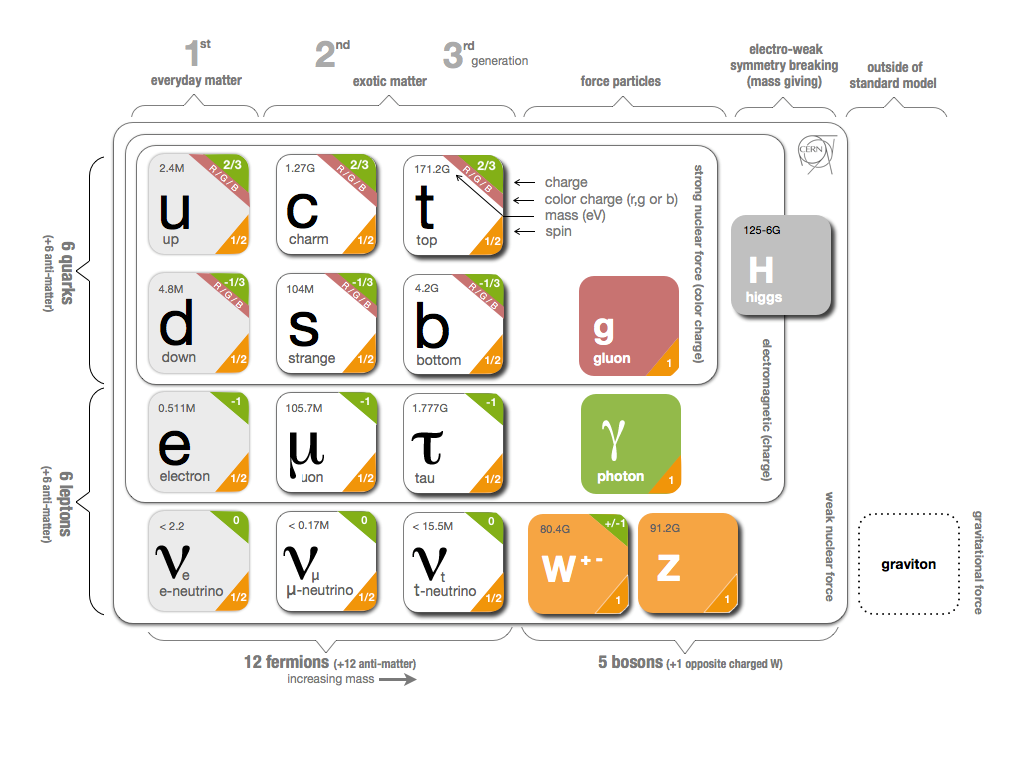
\includegraphics[width=0.8\linewidth]{SM.png}
    \caption{A schematic view of the Standard Model (SM) of the particle physics.}
    \label{fig:intro:SM}
\end{figure}

In general the SM is based on the Yang–Mills theory with local $SU(3)\times SU(2)\times U(1)$ gauge symmetry. It could be divided into several parts:
\begin{itemize}
  \item Quantum chromodynamics sector
  \item Electroweak sector
  \item Higgs sector
  \item Yukawa sector
\end{itemize}

In context of current thesis the electroweak sector is the most interesting. It is based on the group $U(1)\times SU(2)_L$. It mean that we well have two generators: the weak hypercharge ($Y_W$) for $U(1)$ and Pauli matrices for $SU(2)_L$. Index $L$ mean that it affects only left-chiral fermions.

In the SM fermions are described as a doublets (\autoref{sec:dublet}). For each charged lepton there is an appropriate neutrino. While charged lepton could be either right-handed or left-handed, the neutrino could be only left-handed. This part of theory is based on the empirical observations (\autoref{sec:anti}) and this is strictly fixed in the model. Neutrino could interact with the charge current (CC) or neutral current (NC). The appropriate interaction terms are defined as:

\begin{align}
-\mathcal{L}_{CC}&=\frac{g}{2}\sum_\alpha\bar{\nu_{L\alpha}}\gamma^\mu\ell_{L\alpha}W^+_\mu+h.c. \\ \nonumber
-\mathcal{L}_{NC}&=\frac{g}{\sqrt{2\cos{\theta_W}}}\sum_\alpha\bar{\nu_{L\alpha}}\gamma^\mu\nu_{L\alpha}Z^0_\mu
\end{align}

Thus there is no chance for production or detection of the right-handed neutrino (left-handed anti-neutrino).

\subsection{Neutrino flavors}
After the magnificent confirmation of the Standard Model with discovery of the neutral current and W and Z bosons, it became possible to measure precisely the number of neutrino generations. This analysis became possible with massive production of the Z-bosons on so-called Z-factory such as Large Electron-Positron Collider (LEP) at CERN.

The general idea of the study is to look at the different modes of the Z decays. All the decays could be classified into several groups:

\begin{align}
Z&\to hadrons \nonumber \\
Z&\to \ell^+\ell^- \\
Z&\to \nu\bar{\nu} \nonumber
\end{align}

The total width of the boson decay sums up from these three parts. As width of $Z\to \ell^+\ell^-$ is the same of all charge leptons and $Z\to \nu\bar{\nu}$ is the same for all neutrino types they could be multiplied with an appropriate number:

\begin{equation}
\Gamma_Z=\Gamma(Z\to hadrons)+N_{\ell}\times\Gamma(Z\to \ell^+\ell^-) + N_{\nu}\times\Gamma(Z\to \nu\bar{\nu})
\label{eq:intro:nnu}
\end{equation}

During the experiment the $\Gamma_Z$, $\Gamma(Z\to hadrons)$ and $\Gamma(Z\to \ell^+\ell^-)$ were measured. The equality of the $\Gamma(Z\to e^+e^-)$ and $\Gamma(Z\to \mu^+\mu^-)$ was checked. The width of the decay into neutrons came from the theory. The number of neutrino generations remained the only unknown variable in the~\autoref{eq:intro:nnu}. The results of the precise measurements of the Z-boson resonance and predictions for 2, 3 and 4 neutrino generations are shown in~\autoref{fig:intro:NuGen}. From these studies the $N_{\nu}=2.9840\pm0.0082$. So we could conclude that there are only three types of the left-handed neutrino with masses less than Z-boson mass.

\begin{figure}[!ht]
    \centering
    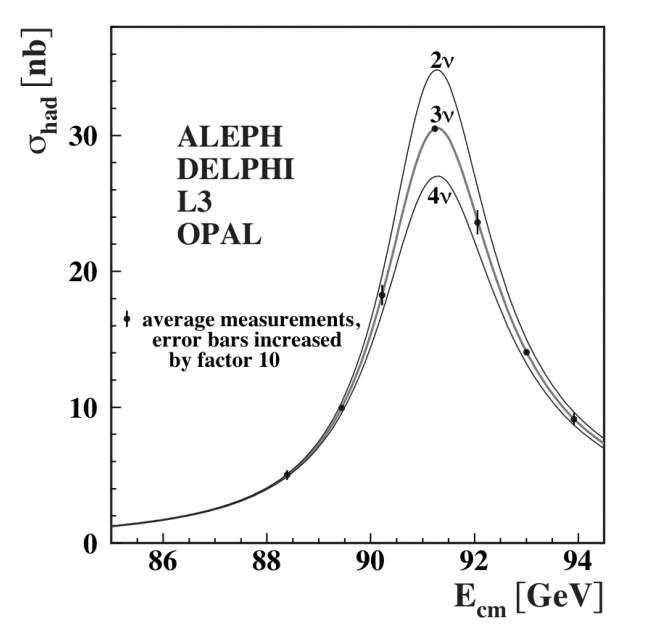
\includegraphics[width=0.6\linewidth]{Neutrino_gen.png}
    \caption{Measurement of the hadron production cross-section as a function of the LEP center-of-mass energy around the Z-boson resonance.}
    \label{fig:intro:NuGen}
\end{figure}


\subsection{Neutrino mass measurements}
In spite of the Standard Model assumption about the neutrino massless nature there were plenty attempts to measure its mass. After the confirmation of the fact that neutrino has mass from neutrino oscillation phenomena (\autoref{sec:osc}) these measurements became essential.

\subsubsection{Beta decay}
The straight-forward way for the neutrino mass measurements is a search for the effect of the nonzero neutrino mass in the beta decay spectrum. One need to measure the energy of outgoing electrons and look at the far end of the distribution. The variation of the neutrino mass change dramatically the energy spectrum in this particular region. For the electron source the deuterium or a tritium isotope is usually chosen. The main technological issues is to perform extremely precise measurements of the electron energy. The most accurate limits obtained with this method for a long time belonged to Mainz~\cite{Kraus2005} and Troitsk~\cite{Aseev2011} experiments. Recently KATRIN experiment announced more precise neutrino mass limits $m_\nu < 1.1 eV$ with 90\%CL.~\cite{Aker2019}.

It's important to notice what is a ``neutrino mass'' $m_\nu$ that is measured in the beta decay.
\begin{equation}
m_\nu\equiv m_\beta\equiv\sqrt{\sum_i\left|U_{ei}\right|^2m_i^2}
\end{equation}

More details about the neutrino mixing will be presented in~\autoref{sec:osc}.

\subsubsection{Neutrinoless double beta decay}
In case neutrino has a Majorana nature it's possible to measure the $m_{ee}$.
\begin{equation}
m_{ee}=\sum_i U^2_{ei}m_i
\end{equation}

All the $0\nu\beta\beta$ experiments are putting the limits of the current value. The most precise result was obtained by KamLAND-Zen experiment $m_\beta\beta < (61-165) meV$ 90\% C.L.~\cite{Gando2016}. One should keep in mind that successful measurement possible only in case of Majorana neutrino nature.

\subsubsection{Cosmology}
Cosmology

Sn1987
Plank


\section{Neutrino oscillations}
\label{sec:osc}

\subsection{Theory}

\subsection{Experiment overview}
\label{sec:exp}



\section{Prospects of the neutrino physics}





\chapter{HNL analysis motivation}
\label{ch:intro:HNL}

As presented in the \autoref{sec:osc} during the exploration of the neutrino oscillation phenomenon, non-zero difference between neutrino eigenstates was observed. That leads to the conclusion that at least two of the three eigenstates should be massive. While in the SM the neutrinos are massless (\autoref{sec:sm}). The theory explaining the mass origin of the neutrino is required.

The easiest solution is try to implement the same process that gives mass to all other particles in the SM --- Higgs mechanism~\cite{Higgs1964} (also called Englert–Brout–Higgs–Guralnik–Hagen–Kibble mechanism for all contributed scientists). There are several problems on this way:
\begin{itemize}
  \item the scale of the neutrino mass is very different from the other particles in the SM. The neutrino masses are less then 1 eV~\cite{Aker2019}, while the other particles mass scale is around 1 MeV, that gives us a difference of 6 orders. It could be event larger up to 8 orders in case of minimum possible neutrino mass. It's hard to believe that the same mechanism is responsible of the generation of mass at so different scales.
  \item as described in the~\autoref{sec:anti} only left-handed neutrinos and right-handed anti-neutrinos were observed. While for the Higgs mechanism both left and right handed particles are required.
\end{itemize}

That leads to the fact that we need to implement some new mechanism or/and new fundamental particles to explain the origin of the neutrino masses.



\section{Theory}

\subsection{Motivation}

\subsection{Prospects}


\section{Experiments and challenges}

\end{document}